\documentclass[letterpaper]{article}
%\documentclass[12pt,letterpaper]{article}
%\setlength{\textwidth}{480pt}
%\setlength{\textheight}{630pt}
%\setlength{\voffset}{0pt}

\usepackage{amsmath, geometry, graphicx, tikz}
\usetikzlibrary{arrows.meta}
\bibliographystyle{plain}

\title{Variation of Genomic Imprinting in the Human Brain}
%\title{Regulators and Psychiatric Associates of Genomic Imprinting in the Human Brain}
\author{Attila Guly\'{a}s-Kov\'{a}cs\(^\ast\), Ifat Keydar\(^\ast\),
...,
%\\
%Eva Xia, Menachem Fromer, Doug Ruderfer,\\
%Ravi Sachinanandam,
Andrew Chess}
\date{Mount Sinai School of Medicine}

\begin{document}

\maketitle

\begin{abstract}
We present a
genome-wide analysis of human genomic imprinting based on
RNA-seq measurements of
parental bias in allele-specific expression in the
dorsolateral prefrontal cortex.  We find that the fraction of imprinted human
genes is consistent with lower (\(\approx 0.5\%\)) as opposed to higher
(\(\approx 5\%\)) estimates in mice.  Our analysis reveals that age up or
down-regulates allelic bias of some, but not all, imprinted genes
in adulthood
and
that allelic bias depends also on genetic variation.
These results support the
hypothesized role of imprinted genes in social interactions, which dynamically
change in the life course and depend on neuropsychological function.
\end{abstract}

\section{Introduction}

Genomic imprinting, leading to repression of either the maternal or paternal
allele, has reached its highest prevalence in humans and other placental
organisms~\cite{Renfree2012}.  In line with this, well-known physiological
functions of imprinted genes include embryonic and placental development, body
growth, suckling, and maternal behavior~\cite{Plasschaert2014,Peters2014}.
Genomic imprinting requires the placement of different epigenetic marks, such
as DNA methylation, at the respective alleles residing on the chromosomes
originating from the mother or father~\cite{Plasschaert2014}.  Indeed,
imprinted genes typically reside in clusters spanning hundreds of kilobases
and allele-specific differential epigenetic marks are found near specific
genes as well as in shared regulatory elements called imprinting control
regions. For non-imprinted genes expression is balanced such that the two
alleles are roughly equally expressed. By contrast, for imprinted genes
epigenetic marks lead to substantial degrees of
imbalance in the expression level of the two alleles.  We refer to the degree
of expression imbalance as \emph{allelic bias}; at its maximum expression is
completely monoallelic.

Why natural selection favors allelic bias for imprinted genes remains
debated~\cite{Wilkins2003,McDonald2005,Keverne2015} but the most mature of all
theories, kinship or conflict theory~\cite{Wilkins2003}, provides a flexible
framework for interpreting past studies on imprinted genes and formulating
hypotheses and predictions regarding their detailed regulation and
physiological function.  The theory assumes that all imprinted genes contribute to
inter-individual interactions in a highly dose-dependent fashion, and explains
allelic bias with the conflicting interests of paternal and maternal genes,
which arise from sexual asymmetries in those interactions~\cite{Wilkins2003}.
A well-known asymmetry is the disproportionate role of mothers in
nurturing offspring in Placentalia.  Kinship theory thus explains why
overexpression disorders of paternally or maternally biased genes in children
abnormally promote or inhibit, respectively, their
growth~\cite{Plasschaert2014,Peters2014}.

Since different inter-individual interactions take place in various
developmental stages and are mediated by various organs, kinship theory
explains the non-uniform pattern of ``imprintedness'' and allelic bias over
various ages~\cite{Bourke2007} and tissue types, which is seen for several
imprinted genes~\cite{Plasschaert2014,Peters2014}.  For other genes such
patterns await discovery.  The theory quantitatively predicts relaxation of
allelic conflict with age~\cite{Ubeda2012} and so raises the hypothesis that
change in allelic bias is linked to aging.  A study on newborn and young adult mice
partially supports that hypothesis~\cite{Perez2015} but experimental evidence
from humans, including older individuals, is missing.

In the framework of kinship theory the question of aging is closely tied to
the roles of imprinted genes in social interactions and in the underlying
psychiatric functions~\cite{Ubeda2012,Wilkins2003}, whose importance has been
increasing in human evolution.  Indeed, most human imprinted gene syndromes
are characterized by not only growth disorder but also mental retardation and
psychiatric dysfunction~\cite{Plasschaert2014,Peters2014}.  More precisely,
paternally and maternally biased genes are suggested to play antagonistic
roles not only in growth but also in psychiatric functions~\cite{Crespi2008a},
since overexpression of the former is associated with autistic while that of
the latter with psychotic spectrum disorders.  For example, maternally derived
microduplications at 15q11-q13 may not only cause the Prader-Willi
syndrome~\cite{Peters2014}---whose symptoms include obesity---but also highly
penetrant for schizophrenia~\cite{Ingason2011,Sullivan2012}, which is perhaps the most devastating
psychotic spectrum disorder.

Recently the CommonMind Consortium produced and
shared\footnote{www.commonmind.org} genome-wide data sets on genotype and gene
expression in the dorsolateral prefrontal cortex (DLPFC) of hundreds of
schizophrenic and control individuals, and identified some 650 differentially
expressed genes~\cite{Fromer2016a}. Our present work extends that analysis
with a focus on allele-specfic expression across the genome, allowing us to
determine allelic bias for each gene.  Based on that, we find that \(\approx
0.6\%\) of all genes are imprinted in the human DLPFC, the majority of which
had been reported to be imprinted in the context of one or another tissue
and/or species. We find a number of genes with allele specific expression
residing near clusters of known imprinted genes. Furthermore, our data suggest
that for several imprinted genes the variation of allelic bias across
individuals is explained by differences in {ancestry and} age in a manner that
depends on the gene.

\section{Methods}

\subsection{Defining the read count ratio to quantify allelic bias}

We quantifieied allelic bias based on RNA-seq reads using a statistic called
\emph{read count ratio} \(S\), whose definition we
based on the total read count \(T\) and the \emph{higher read count} \(H\),
i.e.~the count of reads carrying only either the reference or the alternative SNP variant,
whichever is higher.  The
definition is
\begin{equation}
S_{ig} = \frac{H_{ig}}{T_{ig}}= \frac{\sum_s H_s}{\sum_sT_s},
\label{eq:S-definition}
\end{equation}
where \(i\) identifies an individual, \(g\) a gene, and the summation runs
over all SNPs \(s\) for which gene \(g\) is heterozygous in individual \(i\) (Fig.~\ref{fig:study-design}).
Note that if \(B_{ig}\) is the count or reads that map to the \(b_{ig}\) allele
(defined as above) and if we make the same distributional assumption as above, namely that \(B_{ig}\sim
\mathrm{Binom}(p_{ig}, T_{ig})\), then \(\mathrm{Pr}(H_{ig}=B_{ig}|p_{ig})\), the probability of correctly
assigning the reads with the higher count to the allele towards which
expression is biased, tends to 1 as \(p_{ig} \rightarrow 1\).  We took
advantage of this theoretical result in that we subjected only those genes to
statistical inference, whose read count ratio was found to be high and,
therefore, whose \(p_{ig}\) is expected to be high as well.

Fig.~\ref{fig:study-design} illustrates the calculation of \(S_{ig}\) for the
combination of two hypothetical genes, \(g_1,g_2\), and two individuals,
\(i_1,i_2\).  It also shows an example for the less likely event that the lower rather
than the higher read count corresponds to the SNP variant tagging the higher
expressed allele (see SNP \(s_3\) in gene \(g_1\) in individual \(i_2\)).

Before we carried out our read count ratio-based analyses, however, we cleaned
our RNA-seq data by quality-filtering and by improving the accuracy of SNP
calling with the use of DNA SNP array data and imputation. In the following
subsections of Methods we describe the data, these procedures, as well as our
regression models in detail.

\subsection{Data}

\subsubsection{Brain samples, RNA-seq}

Human RNA samples were collected from the dorsolateral prefrontal cortex of
the CommonMind consortium from a total of \(579\) individuals after
quality control. Subjects included 267 control individuals, as well as 258
with schizophrenia (SCZ) and 54 with affective spectrum disorder (AFF).
RNA-seq library preparation uses Ribo-Zero (which selects against ribosomal
RNA) to prepare the RNA, followed by Illumina paired end library generation.
RNA-seq was performed on Illumina HiSeq 2000.

\subsubsection{Mapping, SNP calling and filtering}

We mapped 100bp, paired-end RNA-seq reads (\(\approx50\) million reads per sample) using Tophat
to Ensembl gene transcripts of the human genome (hg19; February, 2009) with
default parameters and 6 mismatches allowed per pair (200 bp total). We
required both reads in a pair to be successfully mapped and we removed reads
that mapped to \(>1\) genomic locus. Then, we removed PCR replicates using the
Samtools rmdup utility; around one third of the reads mapped (which is
expected, given the parameters we used and the known high repeat content of
the human genome). We used Cufflinks to determine gene expression of Ensembl
genes, using default parameters. Using the BCFtools utility of Samtools, we
called SNPs (SNVs only, no indels). Then, we invoked a quality filter
requiring a Phred score \(>20\) (corresponding to a probability for an
incorrect SNP call \(<0.01\)).

We annotated known SNPs using dbSNP (dbSNP 138, October 2013). Considering all
579 samples, we find 936,193 SNPs in total, 563,427 (60\%) of which are novel.
Further filtering of this SNP list removed the novel SNPs and removed SNPs
that either did not match the alleles reported in dbSNP or had more than 2
alleles in dbSNP. We also removed SNPs without at least 10 mapped reads in at
least one sample. Read depth was measured using the Samtools Pileup utility.
After these filters were applied, 364,509 SNPs remained in 22,254 genes. These
filters enabled use of data with low coverage.  For the 579
samples there were 203 million reads overlapping one of the
364,509 SNPs defined above.  Of those 158 million (78\%) had genotype data
available from either SNP array or imputation.

\subsubsection{Genotyping and calibration of imputed SNPs}

DNA samples were genotyped using the Illumina Infinium SNP array. We used
PLINK with default parameters to impute genotypes for SNPs not present on the
Infinium SNP array using 1000 genomes data.  We calibrated the
imputation parameters to find a reasonable balance between the number of genes
assessable for allelic bias and the number false positive
calls since the latter can arise if a SNP is
incorrectly called heterozygous.

We first examined how many SNPs were heterozygous in DNA calls and had a
discordant RNA call (i.e.~homozygous SNP call from RNA-seq) using different imputation
parameters. Known imprinted genes were excluded. We examined RNA-seq reads
overlapping array-called heterozygous SNPs which we assigned a heterozygosity
score \(L_\mathrm{het}\) of 1, separately from RNA seq data
overlapping imputed heterozygous SNPs, where the \(L_\mathrm{het}\) score could
range from 0 to 1.  After testing different thresholds
we selected an \(L_\mathrm{het}\) cutoff of 0.95 (i.e. imputation confidence
level of 95\%), and a minimal coverage of 7 reads per SNP. With these
parameters, the discordance rate (monoallelic RNA genotype in the context of a
heterozygous DNA genotype) was 0.71\% for array-called SNPs and 3.2\% for
imputed SNPs.

The higher rate of discordance for the imputed SNPs
is due to imputation error.  These were taken into
account in two ways.
First, we considered all imputed SNPs for a gene \(g\) and individual \(i\)
jointly.  Second, we excluded
any individual, for which one or more SNPs supported biallelic
expression.

%At this point, the matrix includes 147
%million data points covering 213,208 SNPs, of which 114 million (77\%) have
%imputation data.

\subsubsection{Quality filtering}

\label{sec:filtering}

Two kind of data filters were applied sequentially: (1) a \emph{read
count-based} and (2) an \emph{individual-based}.  The read count-based filter
removes any such pair $(i,g)$ of individual $i$ and genes $g$ for which the
total read count $T_{ig}<t_\mathrm{rc}$, where the read count threshold
$t_\mathrm{rc}$ was set to 15. The individual-based filter removes any genes
$g$ (across all individuals) if read count data involving $g$ are available
for less than $t_\mathrm{ind}$ number of individuals, set to 25.
These final filtering procedures decreased the number of genes in the data from
\(15584\) to \(n=5307\).

\subsection{Test for nearly unbiased expression}

This test was defined by the criterion
\begin{equation}
S_{ig} \le 0.6 \text{ and } \mathrm{UCL}_{ig} \le 0.7,
\label{eq:unbiased-test}
\end{equation}
where the 95\% upper confidence limit \(\mathrm{UCL}_{ig}\) for the expected
read count ratio \(p_{ig}\) was calculated based on the assumption
that the higher read count \(H_{ig}=S_{ig}T_{ig}\sim \mathrm{Binom}(p_{ig},
T_{ig})\), on the fact that binomial random variables are
asymptotically (as \(T_{ig}\rightarrow \infty\)) normal with
\(\mathrm{var}(H_{ig}) = T_{ig}p_{ig}(1-p_{ig})\), and on the equalities
\(\mathrm{var}(S_{ig}) = \mathrm{var}(H_{ig}/T_{ig}) =
\mathrm{var}(H_{ig})/T_{ig}^2\).  Therefore
\begin{equation}
\mathrm{UCL}_{ig} = S_{ig} + z_{0.975} \sqrt{\frac{S_{ig} (1 - S_{ig})}{T_{ig}}},
\end{equation}
where $z_{p}$ is the $p$ quantile of the standard normal distribution.

\subsection{Regression analysis}
\label{sec:methods-regression}

\subsubsection{Mixed and fixed models}

We modeled the dependence of read count ratio of imprinted genes on biological
and technical explanatory variables (Table~\ref{tab:predictors}) using mixed
and fixed generalized linear models (GLMs).

GLMs in general describe a conditional distribution of a response variable
\(y\) given a linear predictor \(\eta\) such that the distribution is from the
exponential family and that \(\mathrm{E}(y|\eta) = g^{-1} (\eta)\), where
\(g\) is some link function.  In the present context the response \(y\) is the
observed read count ratio that is possibly transformed to improve the model's
fit to the data.  We tested several combinations of transformations, link
functions, and error distributions (Table~\ref{tab:model-names}).  For
inference we used the best fitting combinations as assessed by the normality
(Fig.~\ref{fig:qqnorm-mixed}) and homoscedasticity
(Fig.~\ref{fig:homoscedas-mixed}) of residuals.

In mixed GLMs the linear predictor \(\eta = X
\beta + Z b\) and in fixed GLMS \(\eta = X \beta\), where \(X, Z\) are design
matrices containing data on explanatory variables whereas \(\beta \) and \(b\)
are fixed and random vectors of regression coefficients that mediate fixed and
random effects, respectively (see Section~\ref{sec:mixed-mod} and
Fig.~\ref{fig:glm-vs-hierarch} for 
details).

Besides the random effects term \(Zb\) the key difference between
the mixed and fixed models in this study is that the former describes
read count ratio \emph{jointly} for all imprinted genes and the latter
\emph{separately} for each imprinted gene.  An important consequence is that
our mixed models are more powerful because they can utilize 
information shared by all genes.  Therefore we preferred mixed models for final
inference and used fixed models only to guide selection among possible mixed
models (Section~\ref{sec:fitting}).

\subsubsection{Formulation and interpretation of mixed models}
\label{sec:mixed-mod}

Here we describe the detailed syntax and semantics of the normal linear mixed
models combined with a quasi-log transformation \(Q\) of read count ratio as
this combination was found to provide the best fit
(Fig.~\ref{fig:qqnorm-mixed},~\ref{fig:homoscedas-mixed}).  We have data
on \(579\) individuals and \(30\) imprinted genes and so the response vector is
\(y=(Q_{i_1g_1},...,Q_{i_{579}g_1},Q_{i_1g_2},...,Q_{i_{579}g_2},...,Q_{i_1g_{30}},...,Q_{i_{579}g_{30}})\).
The model in matrix notation is
\begin{eqnarray}
\label{eq:mixed-mod-matrix}
y &=& X \beta + Z b + \varepsilon \\
\varepsilon_i &\overset{\text{i.i.d.}}{\sim}& \mathcal{N}(0, \sigma^2),\;
i=1,...,mn \\
b &\sim& \mathcal{N}(0, \Omega_b),
\end{eqnarray}
where the size of the covariance matrix \(\Omega_b\) depends on the number of
terms with random effects (the columns of \(Z\)).  Simply put: errors and
random coefficients are all normally distributed.

To clarify the semantics of Eq.~\ref{eq:mixed-mod-matrix} let us consider a
simple toy model with just a few terms in the linear predictor.  But before
expressing it in terms of Eq.~\ref{eq:mixed-mod-matrix} it is easier
to cast it in the compact ``R formalism'' of the stats and lme4 packages of the R
language as
\begin{equation}
\label{eq:toy-mod-r}
y \sim \overbrace{1 + \mathrm{Age}}^{\text{fixed effect}} +
\overbrace{\underbrace{(1 + \mathrm{Age} + \mathrm{Ancestry.1} \,|\,
\mathrm{Gene})}_{k=1} +
\underbrace{(1 \,|\, \mathrm{Dx}:\mathrm{Gene})}_{k=2}}^{\text{random
effects}}.
\end{equation}

First note that the random effect term labeled with \(k=1\) can be expanded
into \((1 \,|\, \mathrm{Gene}) + (\mathrm{Age}\,|\, \mathrm{Gene}) +
(\mathrm{Ancestry.1} \,|\, \mathrm{Gene})\).  The `\(1\)'s mean intercept
terms: one as a fixed effect and two as random effects.  The first random
intercept term \((1\,|\,\mathrm{Gene})\) expresses the gene-to-gene
variability in read count ratio (compare panels in Fig.~\ref{fig:S-Dx}
and~\ref{fig:S-age}), in other words the random effect of the
\(\mathrm{Gene}\) variable.  The second random intercept term
\((1\,|\,\mathrm{Dx}:\mathrm{Gene})\) corresponds to the interaction between
psychiatric diagnosis \(\mathrm{Dx}\) and \(\mathrm{Gene}\); it can be
interpreted as the \(\mathrm{Gene}\) specific effect of \(\mathrm{Dx}\)
or---equivalently---as \(\mathrm{Dx}\) specific gene-to-gene
variability.  This term is not likely to be informative as Fig.~\ref{fig:S-Dx}
suggests little \(\mathrm{Gene}\) specific effect of \(\mathrm{Dx}\).

We see that \(\mathrm{Age}\) appears twice: first as a fixed slope effect on \(y\) and
second as a \(\mathrm{Gene}\) specific random slope effect, denoted as
\((\mathrm{Age}\,|\,\mathrm{Gene})\).  The random effect appears to be
supported by Fig.~\ref{fig:S-age} because the dependence of read count ratio
on \(\mathrm{Age}\) varies substantially among genes but the fixed effect is not
supported because the negative dependence seen for several genes is balanced
out by the positive dependence seen for others.  The model includes another
random slope effect: \((\mathrm{Ancestry.1}\,|\,\mathrm{Gene})\) with a
similar interpretation as \((\mathrm{Age}\,|\,\mathrm{Gene})\) but lacks a
fixed effect of \(\mathrm{Ancestry.1}\).

Now we are ready to write the toy model as an expanded special case of
Eq.~\ref{eq:mixed-mod-matrix} as
\begin{equation}
\label{eq:toy-mod-math}
y_{i} = \overbrace{\beta_0 + \mathrm{Age}_{i}
\beta_1}^{\text{fixed effects}} +
\overbrace{\underbrace{b_{0}^{(1)} + \mathrm{Age}_i b_1^{(1)} +
\mathrm{Ancestry.1}_i b_{2}^{(1)}}_{\mathrm{Gene}_i} +
\underbrace{b_{0}^{(2)}}_{\mathrm{Dx}_i:\mathrm{Gene}_i}}^{\text{random
effects}} + \varepsilon_i.
\end{equation}

As in the earlier R formalism the terms of the linear predictor
are grouped into fixed and random effects.  Within the latter group we have
two batches of terms indicated by the \(k\) superscripts on the random
regression coefficients \(b_j^{(k)}\).  The first batch
\(\{b_0^{(1)},b_1^{(1)},b_2^{(1)}\}\) corresponds to
\(\{(1\,|\,\mathrm{Gene}), (\mathrm{Age}\,|\,\mathrm{Gene}),
(\mathrm{Ancestry.1}\,|\,\mathrm{Gene})\}\) in Eq.~\ref{eq:toy-mod-r}, the
second batch contains only \(b_0^{(2)}\) corresponding to
\((1\,|\,\mathrm{Dx}:\mathrm{Gene})\).

Within the \(k\)th batch Eq.~\ref{eq:toy-mod-math} contains only a single
intercept coefficient \(b_0^{(k)}\) and, if random slope terms are also
present in the batch, only a single slope coefficient associated with the
variable \(\mathrm{Age}\) or \(\mathrm{Ancestry.1}\).  This is because only a
single level of the factor \(\mathrm{Gene}\) or the composite factor
\(\mathrm{Dx}:\mathrm{Gene}\) needs to be considered for the \(i\)th
observation; these levels are denoted as \(\mathrm{Gene}_i\) and
\(\mathrm{Dx}_i:\mathrm{Gene}_i\), respectively.  Implicitly however,
Eq.~\ref{eq:toy-mod-math} contains the respective coefficients for all levels
of these factors.  For example, there are \(n=30\) intercept coefficients
\(b_j^{(1)}\) each of which corresponds to a given gene.  So to generalize
Eq.~\ref{eq:toy-mod-math} we need \(J_k\) coefficients in the \(k\)th batch,
where \(J_k\) is the product of the number of factor levels and one plus the
number of random slope variables.  This way we can provide the expansion of
the general formula Eq.~\ref{eq:mixed-mod-matrix} using the semantics of the
toy model (Eq.~\ref{eq:toy-mod-r},~\ref{eq:toy-mod-math}) as
\begin{equation}
y_i = \overbrace{\sum_{j=0}^J x_{ij} \beta_j}^{\text{fixed effects}} +
\overbrace{\sum_{k=1}^K \sum_{j=0}^{J_k} z_{ij}^{(k)}
b_{j}^{(k)}}^{\text{random effects}} + \varepsilon_i.
\label{eq:mixed-mod-general}
\end{equation}

%\begin{eqnarray}
%y_{i} &=& \overbrace{\beta_0 + \mathrm{Age}_{i}
%\beta_1}^{\text{fixed effects}} \\
%&+& \overbrace{\underbrace{b_{0}^{(1)} +
%\mathrm{Age}_i b_1^{(1)} +
%\mathrm{Ancestry.1}_i b_{2}^{(1)}}_{\mathrm{Gene}_i} +
%\underbrace{b_{0}^{(2)}}_{\mathrm{Dx}_i,\mathrm{Gene}_i}}^{\text{random effects}} \\
%&+& \varepsilon_i \\
%y &\sim& \overbrace{1 + \mathrm{Age}}^{\text{fixed effects}} \\
%&+& \overbrace{\underbrace{(1 \,|\, \mathrm{Gene}) + (\mathrm{Age} \,|\, \mathrm{Gene}) + (\mathrm{Ancestry.1} \,|\, \mathrm{Gene})}_{k=1} +
%\underbrace{(1 \,|\, \mathrm{Dx}:\mathrm{Gene})}_{k=2}}^{\text{random effects}} \\
%y &\sim& \mathrm{Age} +
%(\mathrm{Age} + \mathrm{Ancestry.1} \,|\, \mathrm{Gene}) +
%(1 \,|\, \mathrm{Dx}:\mathrm{Gene})
%\end{eqnarray}

\subsubsection{Model fitting and selection}
\label{sec:fitting}

\begin{itemize}
\item Eq.~\ref{eq:mixed-mod-general} is general in the sense that it describes
many linear predictors that can be constructed from the explanatory variables
in Table~\ref{tab:predictors}.  By model selection we mean finding the best linear
predictor under some criterion.
\item fitting mixed and non-hierarchical regression models with lme4 and stats
R packages, respectively, convergence
\item fit during search was evaluated using information criteria AUC, as well as
p-value from Chi-squared test on the degrees of freedom that depends on the
term(s) added
\begin{enumerate}
\item find the best overall combination of data transformation and model
family (Figure~\ref{fig:qqnorm-mixed},~\ref{fig:homoscedas-mixed})
\item start the search in the space of linear predictors as near the optimum as possible
\item guide the sequence in which further terms are added
\end{enumerate}
\item many of the terms in the linear predictor that significantly improved model fit are technical ones; including them in the model therefore corrects for a large technical noise
\item the model that was found to fit the best is 
\begin{eqnarray*}
Q &\sim&
\mathrm{RIN} + (1 \,|\, \mathrm{RNA\_batch}) + (1 \,|\, \mathrm{Institution}) + (1 \,|\,
\mathrm{Institution}:\mathrm{Individual}) \\
&+& (1 \,|\, \mathrm{Gene}:\mathrm{Institution}) + (1 \,|\, \mathrm{Gender}:\mathrm{Gene}) \\
&+& (\mathrm{Age} + \mathrm{RIN} + \mathrm{Ancestry.1} + \mathrm{Ancestry.3} \,|\, \mathrm{Gene})
\end{eqnarray*}
\end{itemize}

\section{Results}

\subsection{Genome- and population-wide variation of allelic bias}

A total of \(5307\) genes passed our filters designed to remove genes with
scarce RNA-seq data reflecting low expression and/or low coverage of RNA-seq.
Examining these genes, we performed exploratory statistical analysis based on
the read count ratio statistic \(S_{ig}\), whose results (below) we
interpreted in terms of the variation of allelic bias both across genes \(g\)
and across individuals \(i\).  Note that our later analyses
(Section~\ref{sec:results-regression} and below) used
information not only in \(S_{ig}\) but also in the total read count as well as
in data beyond RNA-seq.

Fig.~\ref{fig:ranking-genes} presents the conditional empirical distribution
of \(S_{\cdot g}\) given each gene \(g\).  Each of the three plots of the
upper half show in a distinct representation the same empirical distributions
based on data for three genes.  The main panels of the lower half present, in
the most compact representation, the distributions based on all data (5307
genes).  Two of the three genes in the upper half, PEG10 and ZNF331, are
\emph{known imprinted} genes in the sense that they had previously been found
imprinted in the context of some developmental stage, species, and tissue type
other than the adult human DLPFC.  The third, AFAP1, has not been reported to be imprinted
in any context.  For all three genes \(S_{\cdot g}\) varies considerably
within its theoretical range \([\frac{1}{2}, 1]\).  This suggests variation of
allelic bias across study individuals, although some component of the
variation of \(S_{\cdot g}\) must originate from technical sources.

To identify imprinted genes based on the read count ratio we
defined the score of each gene \(g\) as the location statistic \(1 -
\mathrm{ECDF}_g(0.9)\), which is the fraction of
individuals \(i\) for whom \(S_{ig}>0.9\).  We ranked all 5307 genes
according to their score shown in the side plots of the lower half of
Fig.~\ref{fig:ranking-genes} as gray filled circles.  Larger green circles
mark the three genes mentioned above.  The heat map of empirical distribution
of \(S_{\cdot g}\) of ranked genes (Fig.~\ref{fig:ranking-genes}, lower left)
suggests that the top \(50\) genes, which constitute \(\approx 1\%\) of all
genes in our analysis, are qualitatively different from the bottom \(\approx
99\%\) suggesting that most of them are imprinted.  Consistent with this, the
top-scoring genes tended to cluster around genomic locations that had been
previously described as imprinted gene clusters (Fig.~\ref{fig:clusters}).

\subsection{Imprinted genes in the adult DLPF cortex}

The set of top scoring 50 genes is highly enriched in known imprinted genes,
marked by blue in Fig.~\ref{fig:top-genes} and in \emph{nearby candidate}
genes (green) defined as being within 1Mb of a known imprinted gene. Within
the top 50, we find 29 such genes; 21 known imprinted genes and eight nearby
candidates.

The remaining 21 genes in the top 50 are separated by \(>1\) Mb from some
known imprinted gene (termed \emph{distant candidates}, red in
Fig.~\ref{fig:top-genes}).  Upon further examination these distant candidate
genes are overwhelmingly likely not imprinted. The primary reason for this
conclusion is that we performed a test to see if there is reference allele
bias for all candidate genes. For any gene (known imprinted, or candidate) the
expectation is that when some allelic bias is detected, that should equally
favor the reference or non-reference allele since for a given individual who
is heterozygous at a given SNP in the genome it is reasonable to assume that
the chances are equal that the mother or that the father has the reference
allele. Most known imprinted genes and the nearby candidates display a
reference/non-reference distribution consistent with a binomial distribution
with a probability of 0.5 for both the reference and non-reference alleles.
However, and in sharp distinction, most distant candidates have distributions
of reference/non-reference that are not consistent with equal probabilities
(see genes marked with ``X'' in Fig.~\ref{fig:top-genes}).  Indeed, for most of
them the distribution is shifted towards the reference allele strongly
suggesting that mistaken genotyping, imputation or a mapping issue led to the
presence of these red genes in the list of the top 50 genes. One could argue
that we should have left these genes out of Fig.~\ref{fig:top-genes}, but we
thought it was important to show them and to indicate the reasons they are set
aside.   Note also, that we also tested the hypothesis for each gene \(g\) and
individual \(i\) that allelic expression is (nearly) unbiased
(Eq.~\ref{eq:unbiased-test}).  The fraction of individuals for which the test
was \emph{not} rejected tends to be much higher for the ``red'' genes in the
top 50 (black bars in Fig.~\ref{fig:top-genes}).

While the shifted distribution of reference/non-reference alleles leads us to
discount the possibility of imprinting, random monoallelic expression is still
a distinct possibility for these candidates as our studies of random
monoallelic expression in mice suggested that a substantial fraction
(\(40-80\%\)) of random monoallelically-expressed genes had a very strong bias
towards monoallelic expression of one of the two alleles \cite{Zwemer2012}.
Moreover, it is worth noting that three of these candidates are from the major
histocompatibility locus (HLA), which is notable for extensive polymorphism
and difficulties with allelic identification. For these three genes we also
analyzed them more thoroughly with HLA-specific methods for determining
haplotype based on RNA-seq \cite{Bai2014a} and genotype data \cite{Zheng2014}.
The high observed read count ratios for HLA genes appear to be driven by
eQTL-like effects, not by random monoallelic expression nor by imprinting
(manuscript in preparation).  Examining all the assessable known imprinted
genes, we find than \(\frac{1}{3}\)rd of them have a low gene score. This
suggests that these genes do not display imprinted expression in the human
adult DLPFC, consistent with many reports in the literature indicating that
known imprinted genes are often imprinted in some but not all tissues.  

In subsequent analysis (below) we also consider UBE3A as
demonstrating allelic bias consistent with imprinting in the context of human
adult DLFPC as evidenced by Fig.~\ref{fig:known-genes} even though its rank
falls outside of the top 50.  Thus, we have thirty genes we consider imprinted in the adult DLPFC.

\subsection{Allelic bias of imprinted genes and schizophrenia}
\label{sec:results-regression}

Given that our sample is comprised of neurotypic individuals (Control) as well as individuals with
schizophrenia (SCZ) and with with affective spectrum disorder (AFF), we explored whether there is
any association between diagnosis and allelic bias of imprinted genes.
Fig.~\ref{fig:S-Dx} compares read count ratio
distribution among control, SCZ and AFF for the 30 imprinted genes and suggests there are no
differences among the three groups.

To further explore the data, we performed statistical inference using mixed
effects models.  With this procedure we quantified the extent the read count
ratio is dependent on diagnosis and other explanatory variables. These
included biological variables namely Age, the first five principal components
of ancestry (Ancestry.1,...,Ancestry.5), Gender and also technical variables
such as RIN, the RNA integrity number (see Table~\ref{tab:predictors} for
complete list).  Our mixed regression models describe the dependence of read
count ratio on some or all of the explanatory variables simultaneously, which
allows the dissection of various biological and technical sources of
variation.  Another benefit of the mixed modeling framework is its power with
respect to global, not gene-specific, parameters because it makes use of
information that is only available when all thirty genes are considered
simultaneously; still, it allows the prediction gene-specific regression
coefficients (Fig.~\ref{fig:glm-vs-hierarch} right).  These benefits however
hinge on the goodness of model fit to the data.  Therefore, we fitted many
alternative mixed models, selected the best-fitting one using the Akaike
Information Criterion (AIC) and confirmed the goodness of fit with diagnostic
plots (Section~\ref{sec:fitting},
Fig.~\ref{fig:qqnorm-mixed},~\ref{fig:homoscedas-mixed}).

Based on the selected, best fitting, model we formally tested whether read count ratio
depends on various predictor terms that represent either the main effect of
some biological variable or the interaction between two variables
(Table~\ref{tab:mod-sel}).  For example, given prior observations as well as
the empirical distribution of data in Figures~\ref{fig:S-Dx}
and~\ref{fig:S-age}, one would expect the model-based test should detect
gene-to-gene variability of read count ratio.  Indeed that variability---more
precisely the random main effect \((1\mid\mathrm{Gene})\) of the Gene
variable---is strongly supported by the test with a \(\Delta
\mathrm{AIC}\) of \(-127\) and a p-value of \(<10^{-27}\)
(Table~\ref{tab:mod-sel}).

Returning to our main question the model-based test did not support any
overall dependence of read count ratio on diagnosis (\(\Delta \mathrm{AIC} =
2.0,\; p = 1.0\) for the random main effect \((1\mid\mathrm{Dx})\)) consistent
with Figures~\ref{fig:S-Dx} and~\ref{fig:S-age}.  A related test for
gene-specific effects of diagnosis, wherein the effect of Dx varies across the
thirty genes, also yielded negative result (\(\Delta \mathrm{AIC} = 0.4,\; p =
0.21\) for the interaction term \((1\,|\,\mathrm{Dx}:\mathrm{Gene})\)), which
is again consistent with Figures~\ref{fig:S-Dx} and~\ref{fig:S-age}.
Together, these analyses indicate that diagnosis of SCZ or AFF does not have a
substantial impact on the extent of allelic bias of imprinted genes in the
DLPFC. 

\subsection{Gene-specific effects of age and ancestry}

Fig.~\ref{fig:S-age} shows that the read count ratio depends negatively on age
for some imprinted genes (e.g.~PEG3, ZNF331), depends positively for other
genes (e.g.~KCNK9, RP13-487P22.1), and is independent of age for the rest of
imprinted genes (e.g.~NDN, NLRP2).  However, any apparent age effect may be
indirect in the sense that it is mechanistically mediated by other explanatory
variables to which age is associated with
(Fig.~\ref{fig:predictor-associations}).

To investigate the direct effect of age we turned to our best fitting mixed
model once again, evaluating how significantly predictor terms associated with
these variables improve the model's fit (Table~\ref{tab:mod-sel}).  As for Dx
we defined two terms for each variable, the term \(\mathrm{Age}\) represents
a fixed effect that is shared by all imprinted genes while the term
\((\mathrm{Age}\,|\,\mathrm{Gene})\) symbolizes random, gene-specific, age effects.
The shared effect was not supported by our criteria of model fit but the
gene-specific effects received strong support at \(\Delta\mathrm{AIC}<-20\)
and \(p<3\times 10^{-5}\), which is consistent with the large gene-to-gene
variation of age dependence suggested by Fig.~\ref{fig:S-age}.

The above result means a significantly greater than zero variance of the
random coefficients that mediate the gene-specific age effect.  We
complemented this with the posterior predicted values of those coefficients
given the data and the estimated variance (Fig.~\ref{fig:pred-rnd-coefs} top
middle).  These predictions showed an overall agreement with the qualitative
findings on age dependence presented in Fig.~\ref{fig:S-age} with some finer
discrepancies (e.g.~UBE3A), which allude to the model's ability to dissect
direct effects from indirect ones.

A similar analysis of the effects of ancestry principal components and gender
gave also similar results: while the fixed effect, shared by all genes, of
these variables was neglectible, three of the random, gene-specific, effects
received significant support.  These three are
\((\mathrm{Ancestry.1}\,|\,\mathrm{Gene})\),
\((\mathrm{Ancestry.3}\,|\,\mathrm{Gene})\) and
\((1\,|\,\mathrm{Gender}:\mathrm{Gene})\) (Table~\ref{tab:mod-sel}).  The
corresponding predicted random coefficients are presented in
Fig.~\ref{fig:pred-rnd-coefs}.

\begin{itemize}
\item TODO: predict the effect of Age that is specific to each gene;
note that similar prediction for Ancestry.1 is possible but seems much less
interesting because we do not know the genetic mechanisms linked to
Ancestry.1
\end{itemize}

\section{Discussion}

\begin{itemize}
\item we identified imprinted genes in adult DLPF cortex using an RNA-seq read count ratio approach
that estimates allelic bias for a given gene and individual
\item the resulting set of imprinted genes is in agreement with this and that
study but contrasts earlier work (Dulac, Gregg)
\item our model-based inference does not support the hypothesis that perturbed allelic bias
of imprinted genes increases the risk of SCZ
\item implications, alternative hypothetical biological mechanisms involving
imprinting and SCZ
\item alternatively the effect exists but has been masked by the large technical noise in our study
\item
we also examined the dependence of allelic bias on variables namely age,
gender and ancestry
\item we find (so far the strongest?) evidence that age regulates imprinted genes in adulthood
\item biological significance in light of kinship theory, social interactions and aging
\item we find a strong Ancestry.1:Gene effect; this shows how genetic (Ancestry.1) and epigenetic (imprinting control region of a given gene) mechanisms act together to shape gene expression
\item even subtle variation in allelic bias and allele specific expression might substantially affect biological function for some (imprinted) genes while not for others; this must be borne in mind in interpreting our results
\end{itemize}

\bibliographystyle{plain}
\bibliography{monoall-ms}

\newpage

\section{Figures, Tables and Supplementary Material}

\begin{table}
\begin{center}
\begin{tabular}{rlrc}
predictor term                              & interpretation&   \(\Delta\)AIC &        p-value \\
\hline
\((1\,|\,\mathrm{Gene})\)                   & variability among genes & \(-126.8\)  & \(8.5\times 10^{-28}\) \\
\((1\,|\,\mathrm{Dx})\)                     & variability among Control, SCZ, AFF & \(2.0\)  & \(1.0\)  \\
\((1\,|\,\mathrm{Dx}:\mathrm{Gene})\)       & Gene specific variability among Ctrl, SCZ, AFF & \(0.4\) &  \(0.21\) \\
\(\mathrm{Age}\)                            & effect of Age & \(1.3\)   & \(0.39\) \\
\((\mathrm{Age}\,|\,\mathrm{Gene})\)        & Gene specific effect of Age & \(-18.9\)  & \(2.5\times 10^{-5}\)  \\
\(\mathrm{Ancestry.1}\)                     & effect of Ancestry.1 & \(0.6\)  & \(0.24\) \\
\((\mathrm{Ancestry.1}\,|\,\mathrm{Gene})\) & Gene specific effect of Ancestry.1 & \(-71.2\)   & \(4.6\times 10^{-16}\) \\
\((1\,|\,\mathrm{Gender})\)                 & difference between Male and Female & \(2.0\)  & \(1.0\)  \\
\((1\,|\,\mathrm{Gender}:\mathrm{Gene})\)   & Gene specific difference between M and F & \(-5.7\) &  \(5.5\times 10^{-3}\) \\
\end{tabular}
\end{center}
\caption{Selected biological terms in the predictor of a mixed model and their impact on model fit.  The
smaller (more negative) \(\Delta \mathrm{AIC}\), and the smaller the p-value,
the more likely that the term has non-zero effect on the read count ratio.
For further discussion on interpretation and mathematical properties of terms see
Section~\ref{sec:mixed-mod}.
}
\label{tab:mod-sel}
\end{table}

\begin{figure}[h]
\begin{center}
\includegraphics[width=1.0\textwidth]{figures/by-me/commonmind-rna-seq-ms/commonmind-rna-seq-ms.pdf}
\end{center}
\caption{ Quantifying allelic bias of expression in human
individuals using the RNA-seq read count ratio statistic \(S_{ig}\).  The strength of
bias towards the expression of the maternal (red) or paternal (blue) allele of
a given gene \(g\) in individual \(i\) is gauged with the count of RNA-seq
reads carrying the reference allele (small closed circles) and the count of
reads carrying an alternative allele (open squares) at all SNPs for which the
individual is heterozygous.  The allele with the higher read count tends to
match the allele with the higher expression but measurement errors may
occasionally revert this tendency as seen for SNP \(s_3\) in gene \(g_1\) in
individual \(i_2\).
%The differences in the unobserved allelic bias
%between individual \(i_1\) and \(i_2\) arise only from biological differences
%such as their disease status (black and gray silhouettes), age, or gender.  In
%addition to these, the differences in the observed read count ratio also
%reflect variation from technical sources like tissue preparation, or RNA
%sequencing. 
}
\label{fig:study-design}
\end{figure}

\begin{figure}[h]
\begin{center}
\includegraphics[scale=0.6]{figures/2016-07-19-genome-wide-S/complex-plot-1.png}
\end{center}
\caption{
Using the read count ratio statistic \(S\) to report on variation of allelic
bias across individuals and genes.  \emph{Upper half}, from top to bottom: (1)
kernel density estimate; (2) the graph of the survival function 1 - ECDF,
where ECDF means empirical cumulative distribution function; note color scale
for heat map and green filled circles marking genes' score; (3) the heat map
representation of the survival function.  \emph{Lower half}, main panels: heat
map of the survival function for all 5307 analyzed genes ranked according to
their score; right side panels: gene score.
}
\label{fig:ranking-genes}
\end{figure}

\begin{figure}[h]
\begin{center}
\includegraphics[scale=0.6]{figures/2016-08-01-ifats-filters/top-ranking-genes-1.pdf}
\caption{
The top 50 genes ranked by the gene score.  The score of gene \(g\) is \(1 -
\mathrm{ECDF}_g(0.9)\), the fraction of individuals \(i\) for which
\(S_{ig}>0.9\) and is indicated by the length of dark blue, dark green or dark
red bars.  Note that the same ranking and score is shown in the bottom half of
Fig.~\ref{fig:ranking-genes}.  The right border of the light blue, light green
and light red bars is at \(1 - \mathrm{ECDF}_g(0.8)\).  The length of the
black bars indicates the fraction of individuals passing the test of nearly
unbiased expression (Eq.~\ref{eq:unbiased-test}).  ``X'' characters next to
gene names indicate reference allele bias, while ``0'' indicate that
reference allele bias could not be determined due to small amount of data.
}
\label{fig:top-genes}
\end{center}
\end{figure}

\begin{figure}[h]
\begin{center}
\includegraphics[scale=0.6]{figures/2016-11-01-plotting-distribution-of-s/S-Dx-strip-1.png}
\caption{
Distribution of read count ratio for control, schizophrenic (SCZ), and
affectic spectrum (AFF) individuals within each gene that has been considered as imprinted in the DLPFC
brain area in this study.
}
\label{fig:S-Dx}
\end{center}
\end{figure}

\begin{figure}[h]
\begin{center}
\includegraphics[scale=0.6]{figures/2016-11-01-plotting-distribution-of-s/S-Dx-age-1.png}
\caption{
Variation of read count ratio with age.  Color codes psychiatric diagnosis
(Dx) consistent with Fig.~\ref{fig:S-Dx}.
}
\label{fig:S-age}
\end{center}
\end{figure}

% Supplementary tables

\setcounter{table}{0}
\makeatletter 
\renewcommand{\thetable}{S\@arabic\c@table}
\makeatother

\begin{table}[h]
\begin{center}
\begin{tabular}{r|l}
explanatory variable & levels\\
\hline
Age &  \\
Institution & [MSSM], Penn, Pitt\\
Gender & [Female], Male\\
PMI & \\
Dx & [Control], SCZ, AFF \\
RIN &  \\
RNA\_batch & [A], B, C, D, E, F, G, H, 0\\
Ancestry.1 & \\
\vdots & \\
Ancestry.5 &  \\
\end{tabular}
\caption{ \emph{Left column:} explanatory variables of read count
ratio.  \emph{Right column:} levels of each factor-valued (i.e.~categorical)
variable.  Square brackets \([...]\) surround the baseline level against
which other levels are contrasted.  \emph{Abbreviations:} PMI: post-mortem
interval; Dx: disease status; AFF: affective spectrum disorder; SCZ:
schizophrenia; RIN: RNA integrity number;
Ancestry.\(k\): the \(k\)-th eigenvalue from the decomposition of genotypes
indicating population structure.}
\label{tab:predictors}
\end{center}
\end{table}

\begin{table}
\begin{center}
\begin{tabular}{ccc}
%\multicolumn{2}{c}{\replaced{link function and error distribution}{regression models}} \\
model family & abbrev. & response var.~\\
\hline
\emph{u}nweighted \emph{n}ormal \emph{l}inear & unlm  & \(S, Q,\) or \(R\) \\
\emph{w}eighted \emph{n}ormal \emph{l}inear & wnlm  & \(S, Q,\) or \(R\) \\
\emph{logi}stic & logi & \(S\) \\
\emph{logi}stic, \(\frac{1}{2}\times\) down-scaled link fun.~& logi2 & \(S\) \\
\end{tabular}
\caption{Fitted regression model families, in which the response variable is the read count ratio with or without some transformation: 
\(S\)---untransformed, \(Q\)---\emph{q}uasi-log-transformed, and
\(R\)---\emph{r}ank-transformed read count ratio.
}
\label{tab:model-names}
\end{center}
\end{table}

% Supplementary figures

\setcounter{figure}{0}
\makeatletter 
\renewcommand{\thefigure}{S\@arabic\c@figure}
\makeatother

\begin{figure}[h]
\begin{center}
\includegraphics{figures/by-me/monoall-dependencies-2/obs-simple-general/obs-simple-general}
\hspace{\fill}
\includegraphics{figures/by-me/monoall-dependencies-2/obs-simple-general-gene-aspec/obs-simple-general-gene-aspec}
\hspace{\fill}
\includegraphics{figures/by-me/monoall-dependencies-2/mixed/mixed}
\end{center}
\caption{ General dependency structures in two fixed effects regression models
(\emph{left}, \emph{middle}) and a mixed effects model (\emph{right}).  In all
three cases the regression coefficients \(\beta_{1g},...,\beta_{3g}\) or
\(\beta_{1g},b_{2g},b_{3g}\) mediate, for a given gene \(g\), probabilistic
dependencies (arrows) between the response variable \(Y_g\) (read count ratio
for \(g\)) and the corresponding explanatory variables \(X_1,...,X_3\).  For
simplicity but without loss of generality only 3 explanatory variables are
depicted.  The model frameworks differ in how the coefficients relate to each
other for a given explanatory variable (or a given \(j\)).  \emph{Left:} there
is no connection among \(\beta_{jg_1},\beta_{jg_2},...\) which means that the
way \(Y_{g}\), the read count ratio for gene \(g\) depends on variable \(X_j\)
is completely separate from how the read count ratio for any other gene \(g'\)
(i.e.~\(Y_{g'}\)) depends on it.  Consequently no information may be shared
among gene-specific models.  \emph{Middle:} In this case
\(\beta_{jg_1}=\beta_{jg_2}=...\equiv\beta_j\) so that all genes are identical
with respect to how their read count ratio depends the explanatory variables.
Thus genes share all information in the data in the sense that the model
forces them to be identical.  \emph{Right:} Hierarchical mixed effects model
where certain dependencies (\(\beta_1\)) are shared among genes while others
(\(\{b_{2g}\}_g, \{b_{3g}\}_g\)) vary across genes.  The variation is controlled by the
variance parameters \(\sigma^2_j\).  In this example there is a single set
\(\{b_{2g}\}_g\) of random coefficients for \(X_2\)---and a similar set for
\(X_3\)---, which are random intercepts.  In general, however, one or more set
of random slope coefficients may also be present.  Given the estimates
\(\hat{\sigma}^2_j\) and the data the gene-specific random coefficients
\(b_{jg}\) can be predicted.  Among the three only this model framework allows
information sharing among genes in a flexible way.  }
\label{fig:glm-vs-hierarch}
\end{figure}

\begin{figure}[h]
\begin{center}
\includegraphics[scale=0.6]{figures/2017-03-08-model-checking/qqplot-families-M3-1.pdf}
\end{center}
\caption{
Checking the fit of wnlm.Q model: analysis of the normality of residuals.
}
\label{fig:qqnorm-mixed}
\end{figure}

\begin{figure}[h]
\begin{center}
\includegraphics[scale=0.6]{figures/2017-03-08-model-checking/scedasticity-families-M3-1.pdf}
\end{center}
\caption{
Checking the fit of wnlm.Q model: analysis of homoscedasticity.
}
\label{fig:homoscedas-mixed}
\end{figure}

\begin{figure}[h]
\begin{center}
\includegraphics[scale=0.6]{figures/2016-08-08-imprinted-gene-clusters/score-genomic-location-1.png}
\end{center}
\caption{
Clustering of top-scoring genes in the context of human DLPFC around genomic locations that
had been previously described as imprinted gene clusters in other contexts.
}
\label{fig:clusters}
\end{figure}

\begin{figure}[h]
\begin{center}
\includegraphics[scale=0.6]{figures/2016-08-01-ifats-filters/known-genes-1.pdf}
\caption{Known imprinted genes ranked by the gene score (dark blue bars).
``Known imprinted'' refers to prior studies on imprinting in the context of
any tissue and developmental stage.  The length of the
black bars indicates the fraction of individuals passing the test of nearly
unbiased expression.}
\label{fig:known-genes}
\end{center}
\end{figure}

\begin{figure}[h]
\begin{center}
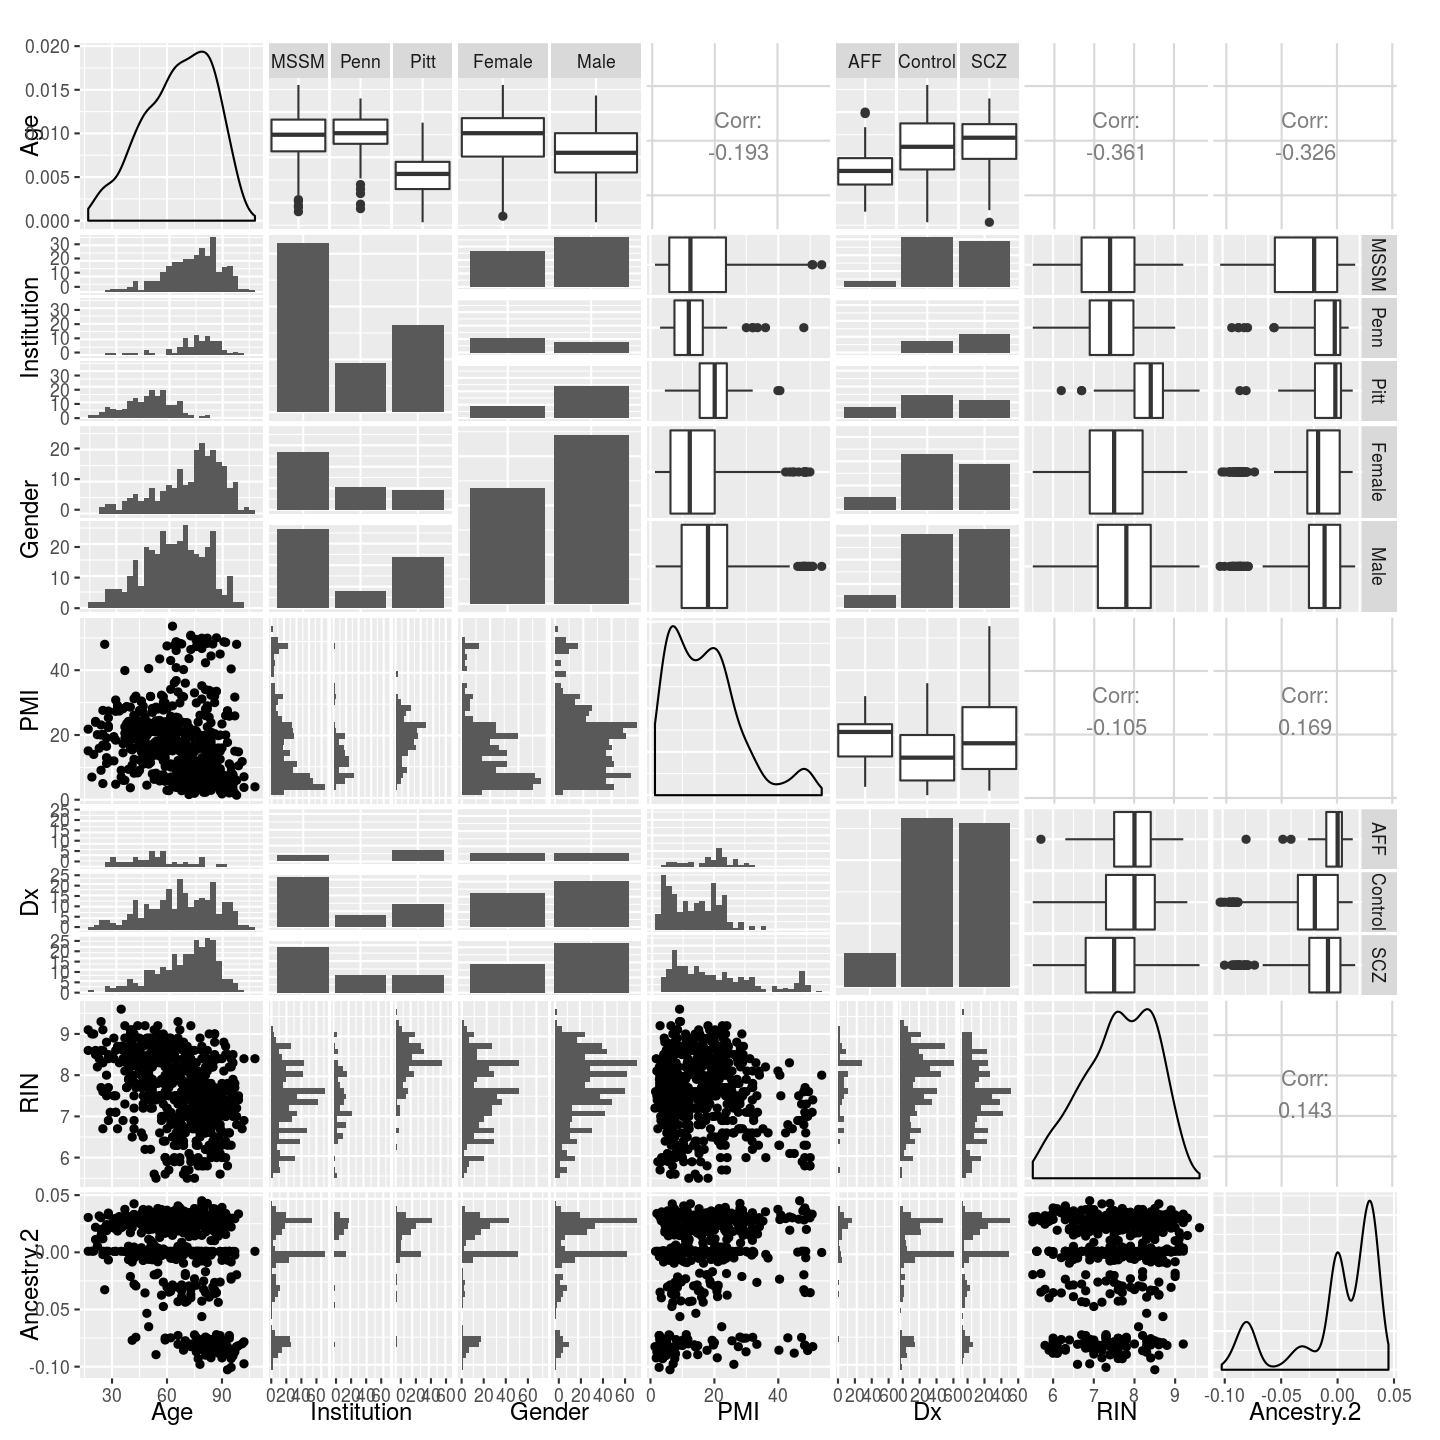
\includegraphics[scale=0.6]{figures/2016-06-26-trellis-display-of-data/evar-scatterplot-matrix-2.png}
\end{center}
\caption{
Distribution and inter-dependence of explanatory variables.  The diagonal graphs of the
plot-matrix show the marginal distribution of six variables (Age,
Institution,...)~while the off-diagonal graphs show pairwise joint
distributions.  For instance, the upper left graph shows that, in the whole
cohort, individuals' Age
ranges between ca.~15 and 105 years and most individuals around 75 years; the
bottom and right neighbor of this graph both show (albeit in different
representation) the joint distribution of Age and Institution, from which can
be seen that individuals from Pittsburg tended to be younger than those from
the two other institutions.
}
\label{fig:predictor-associations}
\end{figure}

\begin{figure}[h]
\begin{center}
\includegraphics[scale=0.6]{figures/2016-06-26-trellis-display-of-data/S-age-gender-1.png}
\caption{
Variation of the read count ratio \(S_{ig}\) with age and gender across hundreds of individuals
\(i\) (dots) and 30 genes \(g\) that have been considered as imprinted in the DLPFC
brain area in this study.
}
\label{fig:S-age-gender}
\end{center}
\end{figure}

\begin{figure}[h]
\begin{center}
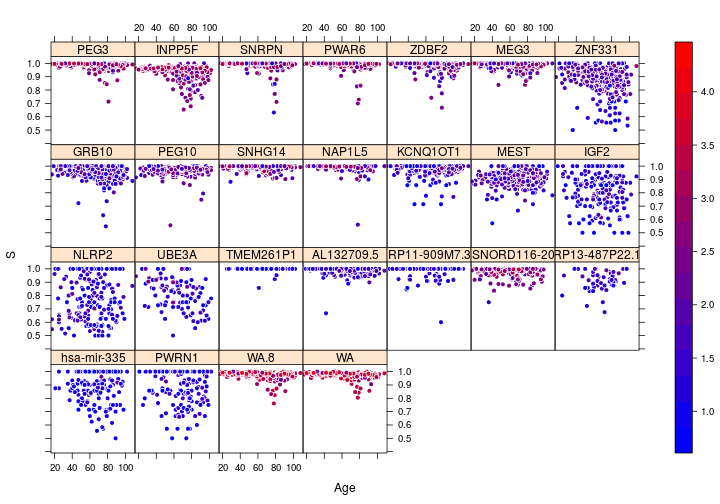
\includegraphics[scale=0.6]{figures/2016-06-26-trellis-display-of-data/S-age-tot-read-count-1.png}
\end{center}
\caption{Variation of total RNA-seq read count across genes and individuals.}
\label{fig:weight-of-evidence}
\end{figure}

\begin{figure}[h]
\begin{center}
\includegraphics[scale=0.6]{figures/2017-07-31-mixed-model-coefs/ranef-gender-gender-gene-m5-all-panels-1.png}
\end{center}
\caption{
}
\label{fig:pred-rnd-coefs}
\end{figure}

\begin{figure}[h]
\begin{center}
\includegraphics[scale=0.6]{figures/2016-10-20-differential-expression-scz/venn-triple-1.pdf}
\end{center}
\caption{
Association of genes' expression to schizophrenia (SCZ) assayed by two RNA-seq
based approaches: total read count (overall expression, Nat Neurosci.~2016
Nov;19(11):1442-1453.)~and read count ratio
(allelic bias, present work).  When these approaches are compared for only
those genes that we find imprinted in the DLPFC in this study, 1 gene is found
associated to schizophrenia by both approaches, 1 by only overall expression,
and 3 by only allelic bias.
}
\label{fig:diff-exp-scz}
\end{figure}

%\begin{figure}[h]
%\includegraphics[width=0.6\textwidth]{figures/2016-10-11-comparison-to-mouse-cerebellum/posterior-pp-vs-pval-wnlm-Q-1.pdf}
%\caption{Comparison of the effects of age and gender between the present work and a
%previous study~\cite{Perez2015} in the mouse cerebellum. }
%\label{fig:mouse-cerebellum}
%\end{figure}

\end{document}
